%%
%% Automatically generated ptex2tex (extended LaTeX) file
%% from Doconce source
%% http://code.google.com/p/doconce/
%%
%-------------------------- begin preamble --------------------------
\documentclass[twoside]{article}
\usepackage{relsize,epsfig,makeidx,amsmath,amsfonts, mathtools}
\usepackage{graphicx}
\usepackage{caption}
\usepackage{subcaption}
\usepackage{fullpage}
\usepackage{listings, color}

\lstset{language=python}
\lstset{basicstyle=\small}
\lstset{backgroundcolor=\color{white}}
\lstset{frame=single}
\lstset{stringstyle=\ttfamily}
\lstset{keywordstyle=\color{red}\bfseries}
\lstset{commentstyle=\itshape\color{blue}}
\lstset{showspaces=false}
\lstset{showstringspaces=false}
\lstset{showtabs=false}
\lstset{breaklines}


% Tricks for having figures close to where they are defined:
% 1. define less restrictive rules for where to put figures
\setcounter{topnumber}{2}
\setcounter{bottomnumber}{2}
\setcounter{totalnumber}{4}
\renewcommand{\topfraction}{0.85}
\renewcommand{\bottomfraction}{0.85}
\renewcommand{\textfraction}{0.15}
\renewcommand{\floatpagefraction}{0.7}
% 2. ensure all figures are flushed before next section
\usepackage[section]{placeins}
% 3. enable begin{figure}[H] (often leads to ugly pagebreaks)
%\usepackage{float}\restylefloat{figure}

\newcommand{\inlinecomment}[2]{  ({\bf #1}: \emph{#2})  }
%\newcommand{\inlinecomment}[2]{}  % turn off inline comments

% insert custom LaTeX commands...

\makeindex

\begin{document}

%-------------------------- end preamble --------------------------





% ----------------- title -------------------------
\begin{center}
{\LARGE\bf INF5620 Final Project}\\
{\LARGE\bf Dynamic linear elasticity}
\end{center}

% ----------------- author(s) -------------------------
\begin{center}
{\bf Ingeborg Sauge Torpe (\texttt{ingebto@math.uio.no})} \\ [3mm]
% List of all institutions:
\centerline{INF5620 - Numerical methods for partial differential equations}
\end{center}
% ----------------- end author(s) -------------------------



% ----------------- date -------------------------
\begin{center}
\today
\end{center}

\vspace{1cm}



\begin{abstract}
This report investigates the dynamic linear elasticity equations using finite differences in time and finite element method in space.
We start by looking at a homogeneous medium, and moves on to look at a heterogeneous medium. 


\end{abstract}

\tableofcontents

\section{Mathematical Problem}
\label{mathproblem}
\index{linear elastcity equation}

We look at the following equations in a unit cube \( \Omega = [0, 1] \times [0, 1] \times [0, 1] \)
\begin{align}
    \rho \mathbf{u}_{tt} &= \nabla \cdot \,\sigma + \rho \mathbf{b} \label{math:elasticity}\\
    \sigma &= 2 \mu \varepsilon(\mathbf{\mathbf{u}}) + \lambda \text{ tr}(\varepsilon(\mathbf{u})) I, \label{math:sigma} \\
    \mathbf{u} &= \mathbf{g} \quad \text{ on } \partial \Omega \\
    \mathbf{u}(\mathbf{x}, 0) &= \mathbf{u}_0 \label{eq_first_init}\\
    \mathbf{u}_t(\mathbf{x}, 0) &= \mathbf{v}_0 \label{eq:sec_init}
\end{align}
where \( \rho\) is the density, \( \sigma\) is the stress tensor, \( \mathbf{b}\) is the body force, tr is the trace and \( \mu\) and \( \lambda\) are Lam\'{e} parameters.
The strain tensor \( \varepsilon\) is defined by \( \varepsilon(\mathbf{u}) = \frac{1}{2} \left( \nabla \mathbf{u} + (\nabla \mathbf{u})^T \right)\).
It is possible to investigate this problem in one, two or three dimensions.
We will look at the three dimensional problem, that is we have \( \mathbf{u} = \mathbf{u}(\mathbf{x}) \; \longmapsto \; \mathbb{R}^d\), with \( d = 3\).



\section{Numerical Solution}
\subsection{Discretization in time using Finite Differences}
\label{timediscretization}
\index{finite difference scheme}
Since we have a time-dependent equation we must discretize both in time and space to get a numerical scheme. 
We choose to use a 2nd order finite difference scheme in time. Then we have
\begin{align}
	\mathbf{u}_{tt} \approx \frac{\mathbf{u}^{n-1} - 2 \mathbf{u}^n + \mathbf{u}^{n+1}}{\Delta t^2}. \label{math:fd}
\end{align}
If we insert (\ref{math:elasticity}) into  (\ref{math:fd}), we obtain a finite difference scheme in time of \(\mathbf{u}\):
\begin{align*}
	\frac{\mathbf{u}^{n-1} - 2 \mathbf{u}^n + \mathbf{u}^{n+1}}{\Delta t^2} \approx \rho \mathbf{u}_{tt} &= \nabla \cdot \,\sigma + \rho \mathbf{b}   \\
	\mathbf{u}^{n+1} &= 2 \mathbf{u}^n - \mathbf{u}^{n-1} + \frac{\Delta t^2}{\rho} \nabla \cdot \,\sigma + \Delta t^2 \mathbf{b} 
\end{align*}




\subsection{Discretization in space using Finite Element Method}
\label{finiteelements}
\index{finite element method}

We shall apply a Galerkin method to the scheme for \( \mathbf{u}^{n+1}\) to obtain the spatial discretization. We use \( \mathbf{v}\) as a test function. We start by looking at the operator 
\begin{align*}
	\mathcal{L}(\mathbf{u}) = \rho \mathbf{u}_{tt} - \nabla \cdot\, \sigma - \rho \mathbf{b}.
\end{align*}
In the means of the Galerkin method, the inner product of this operator with the test function \( \mathbf{v} \in V\) must be zero:
\begin{align}
	(\mathcal{L}(\mathbf{u}), \mathbf{v}) = 0
\end{align}
This leads to the equation
\begin{align*}
	\int_{\Omega} \mathbf{u}^{n+1} \cdot \, \mathbf{v} \, dx &= 2\int_{\Omega} \mathbf{u}^{n} \cdot \, \mathbf{v} \, dx - \int_{\Omega} \mathbf{u}^{n-1} \cdot \, \mathbf{v} \, dx \\
								  &\quad+ \frac{\Delta t^2}{\rho} \int_{\Omega} (\nabla \cdot \, \sigma(\mathbf{u}^{n})) \cdot \, \mathbf{v} \, dx + \Delta t^2 \int_{\Omega} \mathbf{b} \cdot \, \mathbf{v} \, dx 
\end{align*}
We must perform integration by parts in the term with the divergence of \( \sigma\). We get
\(\int_{\Omega} (\nabla \cdot \, \sigma(\mathbf{u}^{n})) \cdot \, \mathbf{v} \, dx 
	=  - \int_{\Omega} \sigma(\mathbf{u}^n) : \nabla \mathbf{v} \, dx + \int_{\partial \Omega} (\sigma(\mathbf{u}^n) \cdot \,\mathbf{n}) \cdot \, \mathbf{v} \, ds\), where the : operator is the tensor matrix product and \( \mathbf{n}\) is the outward pointing unit normal with respect to the surface \( \partial \Omega\). The variational form is then

\begin{align}
	\label{eq:scheme}
	\int_{\Omega} \mathbf{u}^{n+1} \cdot \, \mathbf{v} \, dx = \int_{\Omega} \left( 2\mathbf{u}^{n} - \mathbf{u}^{n-1} + \Delta t^2 \mathbf{b} \right)  \cdot \, \mathbf{v} \, dx - \frac{\Delta t^2}{\rho} \int_{\Omega}  \sigma(\mathbf{u}^n) : \nabla \mathbf{v} \, dx + \frac{\Delta t^2}{\rho}  \int_{\partial \Omega} (\sigma(\mathbf{u}^n) \cdot \,n) \cdot \, \mathbf{v} \, ds
\end{align}
We  write this in a notation introducing an abstract variational statement
written as \( a(\mathbf{u}, \mathbf{v}) = L(\mathbf{v})\), where \( a(\mathbf{u}, \mathbf{v})\) is a so-called bilinear form involving all
the terms containing both the test and trial function, while \( L(\mathbf{v})\) is a linear
form containing all the terms without the trial function. For the equation for \( \mathbf{u}^{n+1}\) we have
\begin{align}
	a(\mathbf{u}, \mathbf{v}) &= \int_{\Omega} \mathbf{u} \cdot \, \mathbf{v} \, dx \\
	L(\mathbf{v}) &= \int_{\Omega} \left( \left( 2\mathbf{u}^{n} - \mathbf{u}^{n-1} + \Delta t^2 \mathbf{b} \right)  \cdot \, \mathbf{v}  - \frac{\Delta t^2}{\rho}  \sigma(\mathbf{u}^n) : \nabla \mathbf{v} \, \right) dx \\
	&\quad+ \frac{\Delta t^2}{\rho}  \int_{\partial \Omega} (\sigma(\mathbf{u}^n) \cdot \,n) \cdot \, \mathbf{v} \, ds
\end{align}



\subsection{Computing 1st time step}
We have derived an explicit scheme for \( \mathbf{u}^{n+1}\) depending on both \( \mathbf{u}^n\) and \( \mathbf{u}^{n-1}\). The initial condition gives us an expression for \( \mathbf{u}^0\), namely
\begin{align*}
	\mathbf{u}(x, 0) = \mathbf{u}_0,
\end{align*}
but we have no expression for \( \mathbf{u}^{-1}\), so we must find a substitution.
We have used a centered difference scheme for the second derivative, so we apply a centered difference scheme for the second initial condition,  given in (\ref{eq:sec_init}), as well:
\begin{align*}
	\mathbf{v}_0 = \mathbf{u}_t(x, 0) \approx \frac{\mathbf{u}^{n+1} - \mathbf{u}^{n-1}}{2\Delta t}
\end{align*}
For \( \mathbf{u}^{n-1}\) we get the following expression
\begin{align}
	\mathbf{u}^{n-1} = \mathbf{u}^{n+1} - 2 \Delta t \mathbf{v}_0
\end{align}
If we insert this to our scheme, (\ref{eq:scheme}), we get
\begin{align*}
	\int_{\Omega} \mathbf{u}^{1} \cdot \, \mathbf{v} \, dx 
		&= \int_{\Omega} \left( \mathbf{u}_{0} + \Delta t \mathbf{v}_0 + \frac{\Delta t^2}{2} b \right)  \cdot \, \mathbf{v} \, dx 
			- \frac{\Delta t^2}{2 \rho} \int_{\Omega}  \sigma(\mathbf{u}_0) : \nabla \mathbf{v} \, dx \\
			&\quad+ \frac{\Delta t^2}{\rho}  \int_{\partial \Omega} (\sigma(\mathbf{u}_0) \cdot \,n) \cdot \, \mathbf{v} \, ds
\end{align*}

The system we have derived are:
\begin{align}
	a_0(\mathbf{u}, \mathbf{v}) &= \int_{\Omega} \mathbf{u} \cdot \mathbf{v} \, dx \\
	L_0(\mathbf{v}) &= \int_{\Omega} \mathbf{u}_0 \cdot \mathbf{v}\, dx \\
	a_1(\mathbf{u}, \mathbf{v}) &= \int_{\Omega} \mathbf{u} \cdot \mathbf{v} \, dx \\
	L_1(\mathbf{v}) &=  \int_{\Omega} \left( \mathbf{u}_{0} + \Delta t \mathbf{v}_0 + \frac{\Delta t^2}{2} \mathbf{b} \right)  \cdot \, \mathbf{v} \, dx - \frac{\Delta t^2}{2 \rho} \int_{\Omega}  \sigma(\mathbf{u}_0) : \nabla \mathbf{v} \, dx + \frac{\Delta t^2}{\rho}  \int_{\partial \Omega} (\sigma(\mathbf{u}_0) \cdot \,n) \cdot \, \mathbf{v} \, ds \\
	a(\mathbf{u}, \mathbf{v}) &= \int_{\Omega} \mathbf{u} \cdot \, \mathbf{v} \, dx \\
	L(\mathbf{v}) &= \int_{\Omega} \left( 2\mathbf{u}^{n} - \mathbf{u}^{n-1} + \Delta t^2 \mathbf{b} \right)  \cdot \, \mathbf{v}  -  \frac{\Delta t^2}{\rho}  \int_{\Omega}\sigma(\mathbf{u}^n) : \nabla \mathbf{v} \,  dx + \frac{\Delta t^2}{\rho}  \int_{\partial \Omega} (\sigma(\mathbf{u}^n) \cdot \,n) \cdot \, \mathbf{v} \, ds
\end{align}


\subsection{Derive linear system}
The obtained equations can be written as a linear system. We then approximate the displacement vector \( \mathbf{u}\) 
\[ \mathbf{\mathbf{u}}^n(x_1, \dots, x_N) = \sum_{j = 0}^{N}\mathbf{c}_j^n \phi_j, \]
where \( \mathbf{c}_j^n, \; j = 0, \cdots, N\) are coefficient vectors and \( \phi_j\) are prescribed finite element basis functions.
If we let \( \mathbf{v} = \varphi_i\), then our scheme can be written 
\begin{align*}
	\int_{\Omega} \left(\sum_{j = 0}^{N}\mathbf{c}_j^{n+1} \phi_j\right) \varphi_i \, dx 
		&= \int_{\Omega} \left( 2\left(\mathbf{c}_{j = 0}^{N}\mathbf{c}_j^n \phi_j\right) - \left(\sum_{j = 0}^{N}\mathbf{c}_j^{n-1} \phi_j\right) 
		+ \Delta t^2 \left(\sum_{j = 0}^{N}b_j^n \phi_j\right) \right)  \varphi_i  \\
		&\quad-  \frac{\Delta t^2}{\rho}  \int_{\Omega}\sigma\left(\left(\sum_{j = 0}^{N}\mathbf{c}_j^n \phi_j\right)\right) : \nabla \varphi_i \,  dx 
		+ \frac{\Delta t^2}{\rho}  \int_{\partial \Omega} \left(\sigma\left(\sum_{j = 0}^{N}\mathbf{c}_j^n \phi_j\right) \cdot \,n\right) \cdot \, \varphi_i \, ds\\
	\sum_{j = 0}^{N} \left( \int_{\Omega} \varphi_j \varphi_i \, dx \right) \mathbf{c}_j^{n+1} 
			&=  2\sum_{j = 0}^{N} \left( \int_{\Omega} \varphi_j \varphi_i \, dx \right) \mathbf{c}_j^{n}
			- \sum_{j = 0}^{N} \left( \int_{\Omega} \varphi_j \varphi_i \, dx \right) \mathbf{c}_j^{n-1} \\
			&\quad+ \Delta t^2 \sum_{j = 0}^{N} \left( \int_{\Omega} \varphi_j \varphi_i \, dx \right) \mathbf{b}_j^{n} 
			- \frac{\Delta t^2}{\rho}\sum_{j = 0}^{N} \left( \int_{\Omega} \sigma(\varphi_j): \nabla \varphi_i \, dx \right) \mathbf{c}_j^{n} \\
			&\quad+ \frac{\Delta t^2}{\rho} \sum_{j = 0}^{N} \left( \int_{\partial \Omega} (\sigma(\varphi_j) \cdot \,n) \cdot \, \varphi_i \, ds \right) \mathbf{c}^n\\
	M \mathbf{c}^{n+1} &= \left(2 M + \frac{\Delta t^2}{\rho}P\right) \mathbf{c}^n - M \mathbf{c}^{n-1} + \Delta t^2 M b^n - \frac{\Delta t^2}{\rho} K \mathbf{c}^n
\end{align*}
We obtain the linear system 
\begin{align}
	M\mathbf{c}^{n+1} = \left(2M + \frac{\Delta t^2}{\rho}(P-K)\right) \mathbf{c}^n - M\mathbf{c}^{n-1} + \Delta t^2 Mb^n,
\end{align}
where \( M_{i, j} = \int_{\Omega} \varphi_j \varphi_i \, dx \), \( P_{i, j} = \int_{\partial \Omega} (\sigma(\varphi_j) \cdot \,n) \cdot \, \varphi_i \, ds\) and \( K_{i,j} = \int_{\Omega} \sigma(\varphi_j): \nabla \varphi_i \, dx \). Here \( \mathbf{c}^{n+1}\) are the unknown and \( \mathbf{c}^n\) and \( \mathbf{c}^{n-1}\) are known from either previous time steps or from the initial conditions.

\section{Implementation using FEniCS}
The implementation is done in python using the FEniCS problem solving environment DOLFIN.
\subsection{Algorithm to solve system}
\begin{enumerate}
	\item Define initial condition \( u = u_0\) and store in \( u\_2\)
	\item Define \( a_0, L_0 \) for the first time step
	\item Assemble matrix \( A\) from \( a_0\) and vector \( l\) from \( L_0\)
	\item Solve system \(  AU=l\) and store in \( u\_1\)
	\item Define new \( L\) for the rest of the time steps
	\item Set time step \( \Delta t\)
	\item Set stop time \( T\)
	\item While \( t \leq T\):
	\begin{enumerate}
		\item Assemble vector \( l\) from \( L\)
		\item Apply boundary conditions
		\item Solve \( AU = l\) and store in \( u\)
		\item Set \( t = t + \Delta t\)
		\item Set \( u\_2 = u\_1\)
		\item Set \( u\_1 = u\)
	\end{enumerate}
\end{enumerate}

\section{Verification}
To test the program an exact test case has been used to find the numerical error generated in each time step. 
The exact solution used is the solution of a rod. We have Neuman boundary conditions on all sides of the cube, except from the to sides in the \( yz\)-plane where \( x= 0\) and \( x = L\), where we have Dirichlet conditions. Our problem then looks like:
\begin{align*}
	\rho \mathbf{v}_{tt} &= \nabla \cdot \,\sigma + \rho \mathbf{b}\\
	\mathbf{u} &= \mathbf{g} \quad \text{ on } \Gamma_0 \\
	\mathbf{u} &= \mathbf{f} \quad \text{ on } \Gamma_1 \\
	\nabla \mathbf{u} \cdot \, \mathbf{n} &= 0 \quad \text{ on } \Gamma_2 \\
	\mathbf{u}(\mathbf{x}, 0) &= \mathbf{u}_0 \\
	\mathbf{u}_t(\mathbf{x}, 0) &= \mathbf{v}_0 
\end{align*}
Here \( \Gamma_0\) is the surface of the side of the cube where \( x = 0\), \( \Gamma_1\) is the surface of the side of the cube where \( x = L\), and \( \Gamma_2 = \Gamma \setminus (\Gamma_0 + \Gamma_1) \).
The equation for the rod is given by
\begin{align}
\label{eq:rod_u}
 \mathbf{u}(\mathbf{x}, t) = 
 			\begin{bmatrix}
				t^2 \alpha x \\
				t^2 \gamma y \\
				t^2 \gamma y
			\end{bmatrix},
\end{align}
where \( \alpha\) and \( \gamma\) are constants.
To find \( \sigma\), we start by computing \( \varepsilon\)
\begin{align*}
	\varepsilon(\mathbf{u}) = \frac{1}{2}(\nabla \mathbf{u} + (\nabla u)^T) = \nabla \mathbf{u}, \quad
	\nabla \mathbf{u} = 
			\begin{bmatrix}
				t^2 \alpha    & 0 & 0 \\
				0 & t^2 \gamma & 0 \\
				0 & 0 & t^2 \gamma
			\end{bmatrix}
\end{align*}
We noe find \( \sigma\)
\begin{align}
	\sigma(\mathbf{u}) &= 2 \mu
				\begin{bmatrix}
					t^2 \alpha    & 0 & 0 \\
					0 & t^2 \gamma & 0 \\
					0 & 0 & t^2 \gamma
				\end{bmatrix}
			+ \lambda (t^2 \alpha + t^2 \gamma + t^2 \gamma)
				\begin{bmatrix}
					1    & 0 & 0 \\
					0 & 1 & 0 \\
					0 & 0 & 1
				\end{bmatrix} \nonumber\\
			&= t^2\begin{bmatrix}
					(2\mu + \lambda) \alpha + 2\lambda \gamma   & 0 & 0 \\
					0 & \lambda \alpha + 2(\mu + \lambda) \gamma & 0 \\
					0 & 0 & \lambda \alpha + 2(\mu + \lambda) \gamma
				\end{bmatrix}
\end{align}
We want the rod to be held still at \( x = 0\) and being stretched out in the positive x-direction. So in this  case we get the Dirichlet boundary conditions \( \mathbf{g} = (0, t^2\gamma y, t^2 \gamma z)^T\) and \( \mathbf{f} = (t^2 \alpha x, t^2 \gamma y, t^2 \gamma z)^T\) in the boundary conditions. Using these conditions the we want \( \sigma\) on the form
\begin{align}
	\sigma(\mathbf{u}) = 
			\begin{bmatrix}
				\beta & 0 & 0 \\
				0 & 0 & 0 \\
				0 & 0 & 0
			\end{bmatrix}
\end{align}
and we see that to get this we must have \(\lambda \alpha + 2(\mu + \lambda) \gamma = 0 \), which implies \( \gamma = - \frac{\lambda \alpha}{2(\mu + \lambda)}\). If we multiply \( \alpha\) by a scalar,  the nonzero entry, \( \beta\), in \( \sigma\) should behave also increase/decrease by the same factor. Also notice that \( \nabla \cdot \, \sigma = 0\). 


\subsection{Stationary problem}
To verify the solution technique the program was tested for the stationary case, we look at \( \mathbf{u}(\mathbf{x})\). In this case \( \mathbf{u}_{tt} = \mathbf{0}\). Because the divergence of \( \sigma \) is zero \( \mathbf{b} = \mathbf{u}_{tt} = \mathbf{0}\) To check if the solver is correct we look at \( \sigma\). Running the program \texttt{stationary\_elasticity.py} with \( \alpha = 1.0\) yields the \( \sigma\):
\begin{align*}
\text{sigma}= 
\begin{bmatrix*}[r]
 1.00000299e+00   &  3.07894255e-15  & 3.64989432e-15 \\
   3.07894255e-15  & -8.97468038e-16  & -2.79934934e-17\\
   3.64989432e-15  & -2.79934934e-17  & -1.05680543e-15\\
 \end{bmatrix*}.
\end{align*}
Here we see that all other elements than the \( (1,1)\)-entry are close to being zero, which is what we expected. 
Now, look at the same matrix, but with \( \alpha = 2.0\), we get
\begin{align*}
\text{sigma}= 
\begin{bmatrix*}[r]
  2.00000598e+00 &   6.15788510e-15 &  7.29978864e-15 \\
  6.15788510e-15  & -1.79493608e-15 & -5.59869868e-17 \\
  7.29978864e-15  & -5.59869868e-17 & -2.11361086e-15
 \end{bmatrix*}.
\end{align*}
Again, we see that all entries besides the (1, 1)-entry is approximately zero. If we compare the two nonzero entries, we see that the latter is exactly two times the first one, so we get what we expected.
Since we now the exact solution to this problem we can compute the error after the numerical computations.
When \( \alpha = 1.0\), we get error: \( 2.88657986403e-15\), and in the computations with \( \alpha = 2.0\) we get error: \( 5.77315972805e-15\). If we compare these we see that the error doubles when doubling \( \alpha\). This tells me that \( \alpha\) should not be large. Since the error is close to machine precision I am satisfied with the solution and since \( \sigma\) behaves in the manner we predicted, we conclude that the stationary solver is correct. The source code for this solver can be found in Appendix \ref{stationary}.
\begin{figure}
        \centering
        \begin{subfigure}[h]{0.51\textwidth}
                \centering
                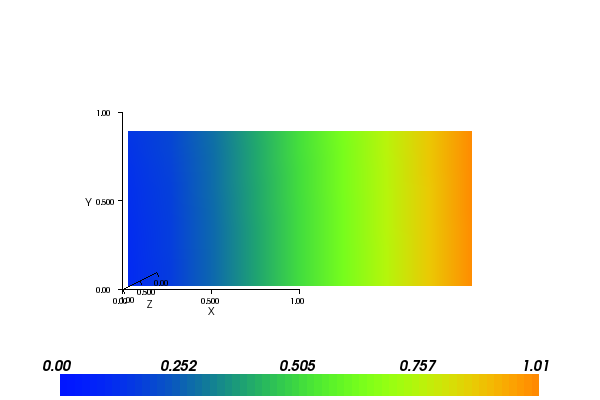
\includegraphics[width=\textwidth]{stat_a=1}
                \caption{\( \alpha = 1.0\)}
                \label{fig:stat_a=1}
        \end{subfigure}%
        ~ %add desired spacing between images, e. g. ~, \quad, \qquad etc. 
          %(or a blank line to force the subfigure onto a new line)
        \begin{subfigure}[h]{0.51\textwidth}
                \centering
                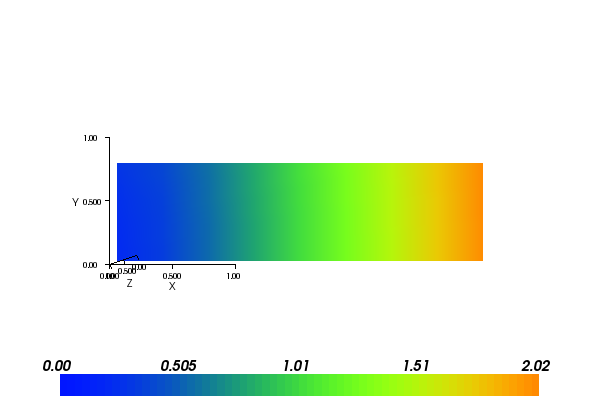
\includegraphics[width=\textwidth]{stat_a=2}
                \caption{\( \alpha = 2.0\)}
                \label{fig:stat_a=2}
        \end{subfigure}
        \caption{Plots showing the displacement of \( \mathbf{u}\) when being streched in the positive x-direction in the stationary case, with two different values of \( \alpha\)}
\end{figure}

\subsection{Test case for time dependent problem}
We now test the stationary solver with our manufactured solution (\ref{eq:rod_u}). We must compute \( b\). Since the divergence of \( \sigma\) is zero \( \mathbf{b} = \mathbf{u}_{tt} = [2\alpha, 2\gamma, 2 \gamma]^T \).
Running simulations in the program \texttt{elasticity.py} we get good results in the first time steps, but after a short while the solution stop being physical, i.e. the material breaks. This might have to do with stability criterion or that the material has been stretched too far. Looking at the maximum error at each time step we see that it increases almost by a factor 10 in each step, which is not good. Running the program with \( \alpha = 1.0\) and \( \rho = 1.0\) with time step \( dt = 0.1\) and stop time \( T = 1.5\) we get the results:
\begin{lstlisting}
Solving linear variational problem.

error after the first time step: 2.42861286637e-17
Solving linear variational problem.

error after time t = 0.2: 3.74700270811e-16
Solving linear variational problem.

error after time t = 0.3: 4.76008121808e-15
Solving linear variational problem.

error after time t = 0.4: 8.66251514964e-14
Solving linear variational problem.

error after time t = 0.5: 2.20232165837e-12
Solving linear variational problem.

error after time t = 0.6: 6.80508982498e-11
Solving linear variational problem.

error after time t = 0.7: 2.04135941484e-09
Solving linear variational problem.

error after time t = 0.8: 6.08751350439e-08
Solving linear variational problem.

error after time t = 0.9: 1.81910732233e-06
Solving linear variational problem.

error after time t = 1: 5.45906540116e-05
Solving linear variational problem.

error after time t = 1.1: 0.00164519066983
Solving linear variational problem.

error after time t = 1.2: 0.0497550422417
Solving linear variational problem.

error after time t = 1.3: 1.50872975643
Solving linear variational problem.

error after time t = 1.4: 45.8363746468
\end{lstlisting}
We see from this that the error becomes bigger than one after time \( t = 1.2\) and from figure \ref{fig:test_t=1.2} and \ref{fig:test_t=1.3} that this is about the same time when the plot stop looking like a rod. It is not completely satisfying to know that the simulations break down and the error increase when as \( t\) increases. But this might be partly be due to the elasticity of the medium, decided by \( \mu \) and \( \lambda\), and the lack of stability criterion for \( dt\). The source code for this solver can be found in Appendix \ref{time}.
\begin{figure}
        \centering
        \begin{subfigure}[h]{0.31\textwidth}
                \centering
                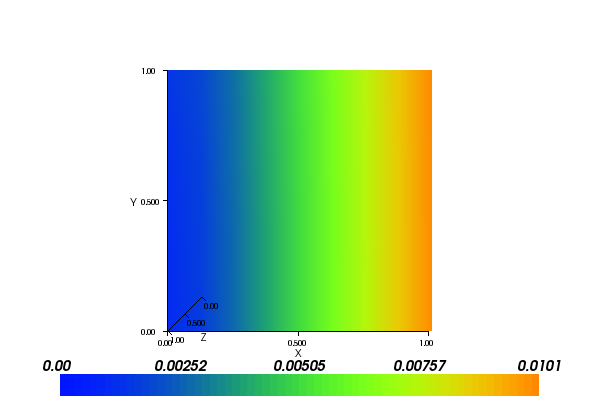
\includegraphics[width=\textwidth]{test_t=01}
                \caption{time \( t = 0.1\)}
                \label{fig:test_t=0.1}
        \end{subfigure}%
        ~ %add desired spacing between images, e. g. ~, \quad, \qquad etc. 
          %(or a blank line to force the subfigure onto a new line)
        \begin{subfigure}[h]{0.31\textwidth}
                \centering
                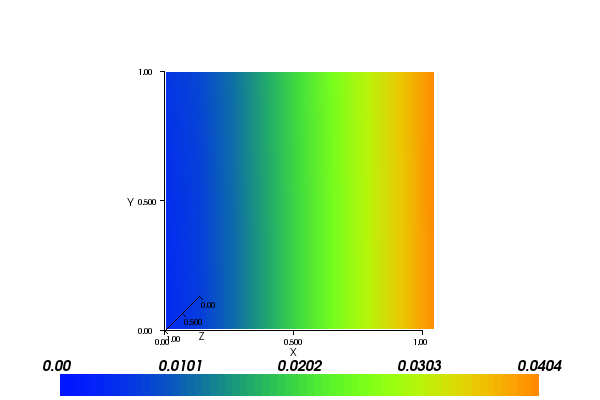
\includegraphics[width=\textwidth]{test_t=02}
                \caption{time \(  t = 0.2\)}
                \label{fig:test_t=0.2}
        \end{subfigure}
        \begin{subfigure}[h]{0.31\textwidth}
                \centering
                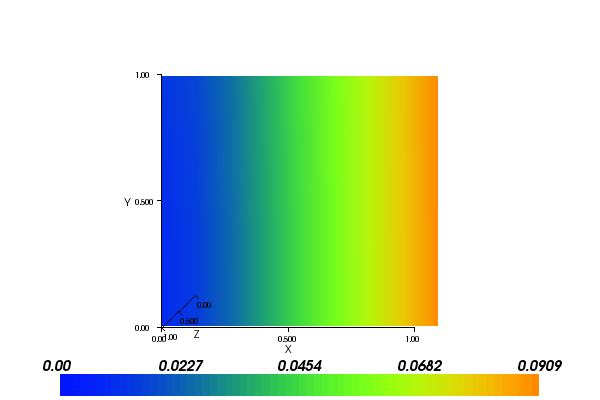
\includegraphics[width=\textwidth]{test_t=03}
                \caption{time \( t = 0.3\)}
                \label{fig:test_t=0.3}
        \end{subfigure}
        
        \begin{subfigure}[h]{0.31\textwidth}
                \centering
                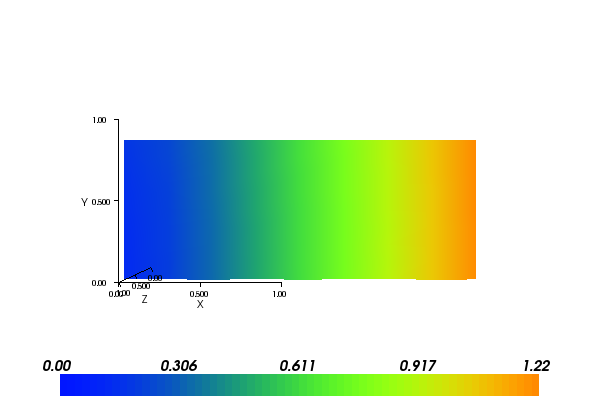
\includegraphics[width=\textwidth]{test_t=11}
                \caption{time \( t = 1.1\)}
                \label{fig:test_t=1.1}
        \end{subfigure}
        \begin{subfigure}[h]{0.31\textwidth}
                \centering
                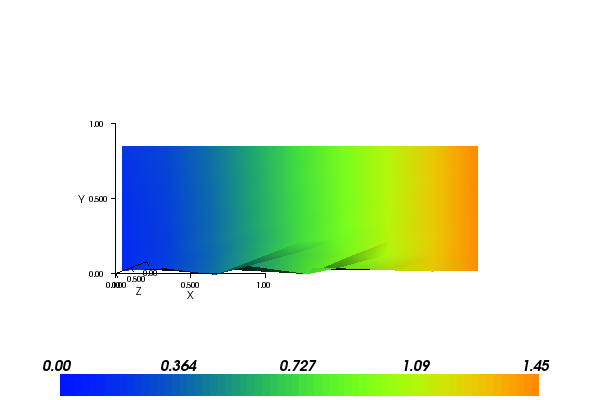
\includegraphics[width=\textwidth]{test_t=12}
                \caption{time \( t = 1.2\)}
                \label{fig:test_t=1.2}
        \end{subfigure}
        \begin{subfigure}[h]{0.31\textwidth}
                \centering
                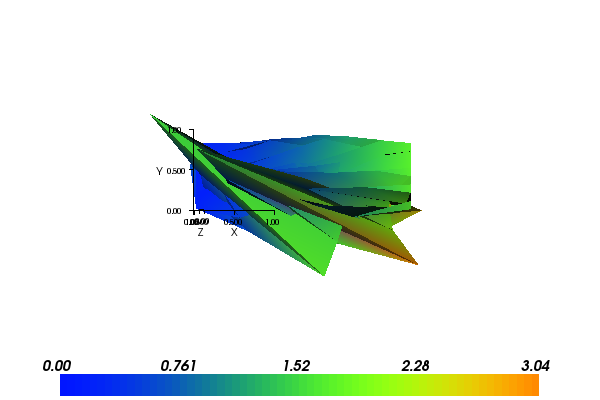
\includegraphics[width=\textwidth]{test_t=13}
                \caption{time \( t = 1.3\)}
                \label{fig:test_t=1.3}
        \end{subfigure}
        \caption{Plots showing the displacement of \( \mathbf{u}\) when being streched in the positive x-direction in the time dependent case, with \( \alpha = 1.0\)}
\end{figure}


\section{Heterogeneous medium}
I have also implemented a solver which handles two different media. This not as well tested as the two other cases, but is built on the stationary solver, so it should give the same results. The problem though, is that when defining the boundary conditions as we have done, and just varying Lam\'{e} elasticity parameters, we get no visible difference. So all in all it seems quite silly to look at two different domains when they behave exactly the same. If I had more time I would definitely found a way to fix this, but because I am out of time this will have to wait. Anyway, the source code can be found in Appendix \ref{heterogeneous_medium}.



\appendix
\section{Source code for the stationary case}
\label{stationary}
\begin{lstlisting}
from dolfin import *
import numpy as np

# Create mesh
elem = 8
mesh = UnitCube(elem, elem, elem)

# Create function space
V = VectorFunctionSpace(mesh, "Lagrange", 1)

# Lame's Elasticity parameters and other constants
E, nu = 1.0, 0.1
mu, lmbda = E/(2.0*(1.0 + nu)), E*nu/((1.0 + nu)*(1.0 - 2.0*nu))
rho = 1.0
alpha = 1.0
gamma = -(lmbda*alpha)/(2*mu + 2*lmbda)

# Create test and trial functions
u, v = TrialFunction(V), TestFunction(V)
n = FacetNormal(mesh)
b = Constant((0.0, 0.0, 0.0))

def  epsilon(u):
	""" Strain tensor """
	#return 0.5*(nabla_grad(u) + transpose(nabla_grad(u)))
	return 0.5*(grad(u) + transpose(grad(u)))

def sigma(u):
	""" Stress tensor """
	return (2*mu*epsilon(u) + lmbda*tr(epsilon(u))*Identity(v.cell().d))

def left_boundary(x, on_boundary):
	tol = 1E-14
	return on_boundary and abs(x[0]) < tol

def right_boundary(x, on_boundary):
	tol = 1E-14
	return on_boundary and abs(x[0] - 1) < tol

# Governing equation
F = inner(sigma(u), grad(v))*dx - rho*dot(b, v)*dx - dot(dot(sigma(u), n), v)*ds
a, L = lhs(F), rhs(F)

# u = [alpha*x, gamma*y, gamma*z]^T
c = Expression(("0.0", "gamma*x[1]", "gamma*x[2]"), gamma = gamma)
r = Expression(("alpha*x[0]", "gamma*x[1]", "gamma*x[2]"), alpha = alpha, gamma = gamma)
bc_l = DirichletBC(V, c, left_boundary)
bc_r = DirichletBC(V, r, right_boundary)
bcs = [bc_l, bc_r]

# Set up PDE and solve
u = Function(V)
problem = LinearVariationalProblem(a, L, u, bcs=bcs)
solver = LinearVariationalSolver(problem)
solver.solve()

exact = Expression(("alpha*x[0]", "gamma*x[1]", "gamma*x[2]"), alpha=alpha, gamma=gamma)
u_e = interpolate(exact, V)
error = np.max(u_e.vector().array() - u.vector().array())
print "\nerror", error

V_ = TensorFunctionSpace(mesh, "Lagrange", 1)
sigma_ = project(sigma(u),V_)
epsilon_ = project(epsilon(u), V_)
matrix = np.zeros((3,3))
q = (elem+1)**3
matrix[0, 0] = sigma_.vector().array()[0*q]
matrix[0, 1] = sigma_.vector().array()[1*q]
matrix[0, 2] = sigma_.vector().array()[2*q]
matrix[1, 0] = sigma_.vector().array()[3*q]
matrix[1, 1] = sigma_.vector().array()[4*q]
matrix[1, 2] = sigma_.vector().array()[5*q]
matrix[2, 0] = sigma_.vector().array()[6*q]
matrix[2, 1] = sigma_.vector().array()[7*q]
matrix[2, 2] = sigma_.vector().array()[8*q]
print "alpha:", alpha
print "sigma: \n",matrix
#print len(sigma_.vector().array())

plot(u, mode="displacement", axes=True)
plot(mesh)
interactive()
\end{lstlisting}


\section{Source code for the time dependent case}
\label{time}
\begin{lstlisting}
from dolfin import *
import numpy as np

# Create mesh
elem = 8
mesh = UnitCube(elem, elem, elem)

# Create function space
V = VectorFunctionSpace(mesh, "Lagrange", 1)


# Lame's Elasticity parameters and other constants
E, nu = 1.0, 0.1
mu, lmbda = E/(2.0*(1.0 + nu)), E*nu/((1.0 + nu)*(1.0 - 2.0*nu))
alpha = 1.0
gamma = -(lmbda*alpha)/(2*mu + 2*lmbda)
rho = 1.0
dt = 0.1

# Create test and trial functions
u, v = TrialFunction(V), TestFunction(V)
n = FacetNormal(mesh)
b = Expression(("2.0*alpha*x[0]", "2.0*gamma*x[1]", "2.0*gamma*x[2]"), alpha=alpha, gamma=gamma)
u0 = Constant((0.0, 0.0, 0.0))
v0 = Constant((0.0, 0.0, 0.0))

def  epsilon(u):
	""" Strain tensor """
	return 0.5*(nabla_grad(u) + transpose(nabla_grad(u)))

def sigma(u):
	""" Stress tensor """
	return (2.0*mu*epsilon(u) + lmbda*tr(epsilon(u))*Identity(v.cell().d))

# Dirichlet boundary conditions on left boundary
def left_boundary(x, on_boundary):
	tol = 1E-14
	return on_boundary and abs(x[0]) < tol

def right_boundary(x, on_boundary):
	tol = 1E-14
	return on_boundary and abs(x[0] - 1) < tol

def update_bc(t=0.0):
	# u = [t^2*alpha*x, t^2*gamma*y, t^2*gamma*z]^T
	c = Expression(("0.0", "t*t*gamma*x[1]", "t*t*gamma*x[2]"), gamma = gamma, t=t)
	r = Expression(("t*t*alpha*x[0]", "t*t*gamma*x[1]", "t*t*gamma*x[2]"), alpha = alpha, gamma = gamma, t=t)
	bc_l = DirichletBC(V, c, left_boundary)
	bc_r = DirichletBC(V, r, right_boundary)
	bcs = [bc_l, bc_r]
	return bcs

def exact(t=0.0):
	u_exact = Expression(("t*t*alpha*x[0]", "t*t*gamma*x[1]", "t*t*gamma*x[2]"), t=t, alpha=alpha, gamma=gamma)
	return u_exact

u_2 = interpolate(u0, V)
u_1 = TrialFunction(V)

# Gorverning equation for the first time step
F = dot(u_1, v)*dx - dot((u_2 + dt*v0 + (dt**2/2.0)*b), v)*dx \
		+ (dt**2/(2.0*rho))*inner(sigma(u_2), nabla_grad(v))*dx \
		- (dt**2/(2.0*rho))*dot(dot(sigma(u_2), n), v)*ds
a, L = lhs(F), rhs(F)

# Set up PDE for first time step and solve
u_1 = Function(V)
bcs = update_bc(dt)
problem = LinearVariationalProblem(a, L, u_1, bcs=bcs)
solver = LinearVariationalSolver(problem)
solver.solve()
# plot(u_1, mode="displacement", axes=True, title="t = %g" %dt)
# interactive()

# Error after the first time step
u_e = interpolate(exact(dt), V)
error = np.max(u_e.vector().array() - u_1.vector().array())
print "\nerror after the first time step:", error

# Governing equation for all other time steps
F = dot(u, v)*dx - (dot((2*u_1 - u_2 + dt**2*b), v) \
		+ (dt**2/rho)*inner(sigma(u_1), nabla_grad(v)))*dx \
		- (dt**2/rho)*dot(dot(sigma(u_1), n), v)*ds
a, L = lhs(F), rhs(F)
u = Function(V)

T = 1.5
t = 2*dt
while t <= T:
	bcs = update_bc(t=t)

	# Set up PDE and solve
	problem = LinearVariationalProblem(a, L, u, bcs=bcs)
	solver = LinearVariationalSolver(problem)
	solver.solve()
	
	# Error after time step t
	u_e = interpolate(exact(t), V)
	error = np.max(u_e.vector().array() - u.vector().array())
	print "\nerror after time t = %g:" %t, error

	# plot(u, mode="displacement", axes=True, title="t = %g" %t)
	# interactive()
	
	t += dt
	u_2.assign(u_1)
	u_1.assign(u)

V_ = TensorFunctionSpace(mesh, "Lagrange", 1)
sigma_ = project(sigma(u),V_)
epsilon_ = project(epsilon(u), V_)
matrix = np.zeros((3,3))

q = (elem+1)**3
matrix[0, 0] = sigma_.vector().array()[0*q]
matrix[0, 1] = sigma_.vector().array()[1*q]
matrix[0, 2] = sigma_.vector().array()[2*q]
matrix[1, 0] = sigma_.vector().array()[3*q]
matrix[1, 1] = sigma_.vector().array()[4*q]
matrix[1, 2] = sigma_.vector().array()[5*q]
matrix[2, 0] = sigma_.vector().array()[6*q]
matrix[2, 1] = sigma_.vector().array()[7*q]
matrix[2, 2] = sigma_.vector().array()[8*q]
print "t=%g sigma: \n" %t,matrix
\end{lstlisting}



\section{Source code for the stationary case with two domains}
\label{heterogeneous_medium}
\begin{lstlisting}
from dolfin import *
import numpy as np

# Create mesh
mesh = UnitCube(8, 8, 8)

# Define a MeshFunction over two subdomains
subdomains = MeshFunction('uint', mesh, 3)

class Omega0(SubDomain):
    def inside(self, x, on_boundary):
        return True if x[1] <= 0.5 else False

class Omega1(SubDomain):
    def inside(self, x, on_boundary):
        return True if x[1] >= 0.5 else False
# note: it is essential to use <= and >= in the comparisons

# Initilize and mark subdomains 
subdomain0 = Omega0()
subdomain0.mark(subdomains, 0)
subdomain1 = Omega1()
subdomain1.mark(subdomains, 1)

V0 = FunctionSpace(mesh, 'DG', 0)
E, nu = Function(V0), Function(V0)
print len(E.vector().array())

print 'mesh:', mesh
print 'subdomains:', subdomains
print "E: ", E
print "nu: ", nu 

# Loop over cells, extract corresponding 
# subdomain number, and fill cell value in mu, lmbda
E_values = [1.0, 5000.0]
nu_values = [0.1, 100.5]
print "len(subdomains.array()):", len(subdomains.array())
for cell_no in range(len(subdomains.array())):
	# print cell_no
	subdomain_no = subdomains.array()[cell_no]
	E.vector()[cell_no] = E_values[subdomain_no]
	nu.vector()[cell_no] = nu_values[subdomain_no]

print "E degree of freedom: ", E.vector().array()
print "len(E)", len(E.vector().array())
print "nu degree of freedom: ", nu.vector().array()
print "len(nu)", len(nu.vector().array())

# plot(subdomains, title = "subdomains") 
# interactive()

# Create function space
V = VectorFunctionSpace(mesh, "Lagrange", 1)

def  epsilon(u):
	""" Strain tensor """
	#return 0.5*(nabla_grad(u) + transpose(nabla_grad(u)))
	return 0.5*(grad(u) + transpose(grad(u)))

def sigma(u):
	""" Stress tensor """
	return (2*mu*epsilon(u) + lmbda*tr(epsilon(u))*Identity(v.cell().d))

def left_boundary(x, on_boundary):
	tol = 1E-14
	return on_boundary and abs(x[0]) < tol

def right_boundary(x, on_boundary):
	tol = 1E-14
	return on_boundary and abs(x[0] - 1) < tol

# Lame's Elasticity parameters and other constants
E, nu = 1.0, 0.1
mu, lmbda = E/(2.0*(1.0 + nu)), E*nu/((1.0 + nu)*(1.0 - 2.0*nu))
rho = 1.0
alpha = 1.0
gamma = -(lmbda*alpha)/(2*mu + 2*lmbda)

c = Expression(("0.0", "gamma*x[1]", "gamma*x[2]"), gamma = gamma)
r = Expression(("alpha*x[0]", "gamma*x[1]", "gamma*x[2]"), alpha = alpha, gamma = gamma)
bc_l = DirichletBC(V, c, left_boundary)
bc_r = DirichletBC(V, r, right_boundary)
bcs = [bc_l, bc_r]


# Define variational problem
u, v = TrialFunction(V), TestFunction(V)
n = FacetNormal(mesh)
b = Constant((0.0, 0.0, 0.0))

# Governing equation
F = inner(sigma(u), grad(v))*dx - rho*dot(b, v)*dx # - dot(dot(sigma(u), n), v)*ds
a, L = lhs(F), rhs(F)

# Set up PDE and solve
u = Function(V)
problem = LinearVariationalProblem(a, L, u, bcs=bcs)
solver = LinearVariationalSolver(problem)
solver.solve()

exact = Expression(("alpha*x[0]", "gamma*x[1]", "gamma*x[2]"), alpha=alpha, gamma=gamma)
u_e = interpolate(exact, V)
error = np.max(u_e.vector().array() - u.vector().array())
print "\nerror", error


plot(u, mode="displacement", axes=True)
# plot(u, mode="displacement", axes=True)
plot(mesh)
interactive()
\end{lstlisting}









\end{document}